\documentclass[12pt,a4paper]{report}

\usepackage[utf8]{inputenc}
\usepackage{tabularx} % extra features for tabular environment
\usepackage{amsmath}
\usepackage{graphicx}
\usepackage{multicol}
\usepackage{setspace}
\usepackage[
    doi=false,
    isbn=false,
    url=false,
    sorting=none
]{biblatex}
\usepackage{fancyhdr}
\usepackage[ruled, vlined]{algorithm2e}
\usepackage[margin=2.5cm]{geometry}
\usepackage{appendix}
\usepackage{verbatim}
\usepackage{caption}
\usepackage{subcaption}
\usepackage{float}
\newcommand{\code}[1]{\texttt{#1}}
\graphicspath{images/}
\addbibresource{references.bib}
\emergencystretch=1em

\pagenumbering{roman}
\begin{document}

\begin{titlepage}
   \begin{center}
        \vspace*{1cm}
        
        
\includegraphics[width=0.4\textwidth]{images/crest.jpg}
        \vspace{2.5cm}
    
        {\Large\textbf{Agent-Based Modelling of Regional Traffic Evacuation Strategies}}
 
        \vspace{2.5cm}
 
        Jamal Rahman\\
        1416458\\
 
        \vspace{0.5cm}
        
        Supervisor: Dr. J. A. Bullinaria
 
        \vspace{0.5cm}
        
        MSci Computer Science
        
        \vspace{0.5cm}
        
        April 2019
 
       \vfill
 
       \vspace{0.8cm}
 
 
       School of Computer Science\\
       University of Birmingham\\
       Birmingham, B15, 2TT\\
 
   \end{center}
\end{titlepage}

\onehalfspacing
\thispagestyle{plain}
\topskip0pt
\vspace*{\fill}
\begin{center}
    \textbf{Abstract}
\end{center}

Memes

\vspace*{\fill}
\pagebreak

\topskip0pt
\vspace*{\fill}
\begin{center}
    \textbf{Acknowledgements}
\end{center}

\noindent
I would first like to express thanks to my project supervisor, Dr John Bullinaria, for his guidance throughout the duration of the project. 

I also want to thank Mia Wright and the wellbeing team at the College of Engineering and Physical Sciences, who have been invaluable in providing support throughout my time at the University.

Lastly, I want to extend my unbounded gratitude to my parents and to Amelia Elgey. Without their support I would not have been able to complete this project.

\vspace*{\fill}
\pagebreak

\tableofcontents
\listoffigures
\listofalgorithms

\chapter{Introduction}
\pagenumbering{arabic}
\label{ch:introduction}
An emergency evacuation is the time-critical migration of people from a dangerous situation to a position of safety. Disasters such as fires, floods, hurricanes and nuclear hazards can call for evacuations of potentially large regions, and studies have shown that an evacuation of greater than 1000 people occurs, on average, every two to three weeks in the USA \cite{SandiaNationalLaboratories2005IdentificationEvacuations,Murray-Tuite2013EvacuationPractice}. As urban environments become increasingly densely populated, regional infrastructure is often found ill-equipped to handle the stress of an evacuation scenario \cite{Pitt2008TheFloods}, and in recent decades eyes have increasingly turned towards the factors that play into evacuation issues \cite{Dow2002EmergingCarolina} such as households evacuating with more cars than necessary, and the region evacuating too quickly leading to crippling congestion on the road network. If we can understand the factors that are at play in an evacuation, authorities and local governments will be able to design schemes for more efficient and successful egress. Practical evacuation drills on a regional scale are expensive, pose ethical issues and are often simply impossible, for this reason researchers have turned to computational simulation. 

\section{Agent-Based Modelling}
Computer simulation of evacuation scenarios historically used top-down modelling techniques. A top-down technique aims to characterise the macroscopic outcome of a phenomenon using general terms. For example, evacuation systems have previously been modelled using fluid dynamics, drawing parallels between an individual in a crowd with a molecule in a wave \cite{Thompson1995APopulations}.
In contrast, a bottom-up model aims to characterise the individual components of a system on a microscopic basis, modelling their actions and allowing their interactions to naturally produce an \textit{emergent} phenomenon. 

Microsimulation is more computationally taxing than macrosimulation, demanding processing time for each agent in the system; however, bottom-up approaches are able to account for \textit{interactions between agents}, a concept that top-down models are unable to replicate. Modelling scenarios by defining the behaviour of the individual agents is referred to as agent-based simulation or agent-based modelling (ABM). For our purposes we shall use the term ABM to describe such a system.

Microscopic simulation of road networks started becoming computationally feasible in the 1990s, beginning a surge of research that attempted, and succeed, to accurately model road traffic \cite{Nagel1992ATraffic}. As computing power increased further, ABM research accelerated rapidly in the 21st century \cite{Bonabeau2002Agent-basedSystems.,Teodorovic2003TransportApproach}.

\section{Overview}
This report describes the formulation, design and implementation of a multi-agent simulation program for traffic-based evacuation scenarios - and experimentally investigates the impact different strategies and scenario effects can have on evacution time.

Chapter \ref{ch:background} will introduce the background behind the field of agent-based modelling, initially from an abstract context and then within the realm of traffic simulation. We will consider how similar evacuation models have been leveraged, to provide an understanding of the problem space wherein this project lies.

The Project Specification section first gives a formal designation of the project aims - thereafter specifying, in explicit terms, the high-level functional requirements of the program, the program capabilities, and the description of fundamental aspects of the simulation itself. Here, we shall have an understanding of what the system does and broadly how it will attempt to do so. 

System design is addressed in Chapter \ref{ch:design}, giving an overview of how the system's components interact with each other.

The Implementation section explores the realisation of core system components. In particular, we cover the framework for moving within road networks, and the associated algorithms that dictate agent behaviours.


\chapter{Background}
\label{ch:background}
A preeminent introduction to ABM is given by Macal and North (2005), which provides a thorough discussion on what defines an agent. In brief, an agent is an entity which acts independently within an environment:

\section{Agents}
Agents are governed by a set of rules which dictate how they react to their environment and to other agents. Some agents have the ability to perceive and store memory of the environment, as well as events within it, and may adapt their behaviour according to their perceptions \cite{Macal2005TutorialSimulation}. An agent need not be realised specifically as a human; a simulated road network will model a vehicle as an agent, and some models may model collections of jointly-acting people, such as families, as agents \cite{Zhang2009Agent-basedEvacuation}. As long as the collective-agent acts as an independent individual this is accepted.

Agent behaviour can be described at different levels of complexity; it is impracticable to describe the full decision making process behind an agent's actions, accounting for a large set of memories and perceptions. Primitive agents may be modelled as finite state machines \cite{Ren2009Agent-BasedEvacuation}, and in some cases a simple behavioural model is built from a statistical estimation of the agent's behaviour \cite{Dawson2011AnManagement}.

ABM's benefits as a simulation technique are due to its natural ability to capture emergence, its parallels to real-world systems, and its flexibility \cite{Bonabeau2002Agent-basedSystems.}. An emergent phenomenon, by definition, cannot be reduced to the sum of its parts as it is the result of interactions that are decided upon at execution time. The parallels between an agent-based model and a real world system are intrinsic, agents are designed to directly mimic real participants' behaviour. Lastly such systems are flexible in scale; it's easy to increase the number of agents, change the environment or tweak the simulation parameters without making any fundamental changes to the model. Because of this, ABM is notorious for excelling at posing `what if' questions and investigating hypothetical scenarios.

\section{Environments}

Careful consideration of the real world must be taken when designing the fundamental architecture of an ABM - most importantly when choosing the agents' environment. Some applications require a minimal environment, such as in a \textit{supply chain model} which sets agents as \textit{factories, retailers, consumers, etc} and allows them to communicate with each other \cite{Macal2006TutorialAgents}. Here the environment need only be the collection of agents themselves. Alternatively environments may take on a more literal representation, providing a spatial description of a physical environment as is more commonly seen when studying ecological and social behaviour \cite{Macal2005TutorialSimulation}.

When simulating physical, ecological, and sociological phenomena, environments typically fall into three categories: continuous, cellular automata (CA) and networked. Continuous representations use a continuous $(x,y)$ coordinate system within which agents act. CA is a discrete environment, chunking space into a grid. CA models make for a trade off between model accuracy and computational ease; agents reside within a grid cell and naturally have eight surrounding cells. This limitation allows for a simple model that is computationally efficient while still approximate of real space. Lastly, many simulation applications can be realised on a network, or graph. Across all environment representations, the timestep of simulation can be adjusted as a trade off between computational load and model accuracy. It comes naturally to model a regional evacuation scenario using a network environment.


\section{Traffic Model}

In ABM, there is no one accepted process for building simulations and running experiments. Numerous approaches are taken to model road networks, and to simulate evacuation scenarios on them. In order to perform research on road network evacuations, a robust agent-based model must first be constructed.

\subsection{Existing Software and Frameworks}

In the field of ABM, regardless of application area, there is a distinct split between commercial systems and programming frameworks. Typically, researchers use frameworks to make new advancements in their respective problem areas, and development studios implement new techniques into user friendly commercial systems, often with government officials in mind as end users.

\subsubsection{CORSIM, VISSIM and Paramics}

CORSIM, VISSIM and Paramics are three commonly used commercial software packages for traffic modelling.

The systems do not greatly differ in functionality, as all three of the systems specialise in producing a highly representative simulation of the roads. Their focus is on such microscopic matters as modelling the dynamics of different classes of vehicle and other low level details that allow them to accurately model the flow of traffic through individual complex intersections, and small networks \cite{Choa2004CORSIMYou}.
CORSIM, VISSIM and Paramics all allow for programming of the simulation parameters, and they provide comprehensive 2D and 3D visualisation features.


\subsubsection{MASON}

For researchers who need to build models from the ground up, none of CORSIM, VISSIM or Paramics are suitable, as the three models are inflexible towards implementing novel strategies. For such demands, frequently used ABM software frameworks include NetLogo, MASON (Multi-Agent Simulator of Neighbourhoods/Networks) and the Repast Suite. Netlogo uses a proprietary scripting language, whereas MASON and Repast provide libraries for working in Java. While  both solutions provide a core simulation engine, data structures for common environment representations, and visualisation tools, Repast was deemed to be unsuitable for this project; rather than import a library of useful code to use in a system, Repast simulations must be run from within the Repast Suite's own program, and Java files can be written to configure the nature of the simulation that is ran from the Repast main suite. Conversely, MASON operates as a typical Java library does, allowing importing of MASON packages to add features into our own programs. An overview of how MASON works within the project is given in Chapter \ref{ch:design}.


\subsection{Environment Representation}
A road network can be represented as a directed graph $G (N,E)$, where $N$ is the set of nodes (junctions) on the network and $E$ the set of edges (road connections) between all junctions. Nodes $n \in N$ have coordinates $(x,y)$ and edges $e \in E$ have corresponding lengths $l$ \cite{Madireddy2011AnManagement}. Edges and nodes may possess additional properties, such as speed limits.

Simulations are often tested on synthetic network topologies, generated to mimic common road patterns \cite{Zhang2009Agent-basedEvacuation}, alternatively researchers can test on a real world road network extracted from GIS data \cite{Chen2006Agent-BasedKeys}.

\subsection{Vehicle behaviour}
A vehicle's goal is to reach a `safe' node, at which point it is deemed to have evacuated successfully. One approach is to define a sub-region of the network to be evacuated, and any node not in this subset is hence in the set of safe nodes. \cite{Chen2008Agent-basedStrategies} Another more common approach is to identify which roads act as exits to the region which is being modelled, and record their corresponding nodes as safe evacuation nodes. \cite{Madireddy2011AnManagement,Dawson2011AnManagement}.

Multiple algorithms exist for modelling driving behaviour. A tried and tested traffic algorithm is the Nagel-Schrekenberg (N-S) cellular automata model\cite{Nagel1992ATraffic,Nagel1998Two-laneApproach}. See Algorithm \ref{alg:NS}. The N-S model is a CA model, which divides the world space into grid cells of the approximate size of a car. At every timestep, agents will accelerate up to the speed limit, unless there is a car in the way, in which case the agent will slow down to not collide with the car in front. All driving behaviours incorporate a random element, to account for the human factor. The N-S model does this by supplying a probability $p$ with which an agent may overbreak and reduce their speed.

\begin{algorithm}
    \KwData{$Cars = (Velocity, Location)$}
    
    \SetKwFunction{Initialise}{InitialiseLocation}
    \SetKwFunction{Next}{DistanceToNextCar}
    
    \While{running}{
        \For{$car\in Cars$}{
            \uIf{$velocity_{car} < speed\_limit$}{
                $velocity_{car} \leftarrow velocity_{car} + 1$\;
            }
            
            \uIf{$\Next{car} < velocity_{car}$}{
                $velocity_{car} \leftarrow \Next{car} - 1$\;
            }
            
            \uIf{with probability p}{
                $velocity_{car} \leftarrow velocity_{car} - 1$\;
            }
            $location_{car} \leftarrow location_{car} + velocity_{car}$\;
        }
    }
    
    \caption{Nagel-Schreckenberg (N-S) driving model}
    \label{alg:NS}
\end{algorithm}

PARAMICS bases its car-following mechanism on the Fritzsche model \cite{Fritzsche1994ASimulation} which characterises five driving modes that dictate the agent behaviour, however the resultant behaviour is largely the same as with the N-S algorithm. 

Recent research has used continuous adaptations of the N-S algorithm, forgoing the limitations applied by CA, or have opted to use very simple approximations of the algorithm \cite{Durak2015OptimizingAlgorithms,Madireddy2011AnManagement}.


\section{ABM Experiments}

With robust digital models able to accurately model the nuance of the physical world, researchers can leverage the emergence of ABM to pose questions about a hypothetical scenario and solve the problems that arise. 

The most important metric in evacuation research is \textit{clearance time}, which is the total time elapsed between the first evacuee leaving their source to the last evacuee reaching their destination \cite{Shendarkar2006CrowdReality,Madireddy2011AnManagement}.

\subsection{Agent Greed}
Zhang, Ukkusuri and Chan (2009) present a model which models the population with varying levels of \textit{greed}. In this context, a greedy agent is one who diverts from their route depending on their perception of their route's level of congestion. The congestion level, $\rho_e$, of an edge $e$ is given by the following relation:

\BlankLine
\begin{equation}
    \rho_e = \frac{Number\, of\, cars\, on\, edge\, e}{length\, of\, edge\, e\, \times\, average\, car\, length}   
\end{equation}
\BlankLine
\BlankLine

Formally, when a greedy agent approaches a junction it makes a judgement on the congestion level of it's originally planned next road. If congestion on the original planned route exceeds a given tolerance limit, the greedy agent will divert its route via the junction's least congested outbound road, and will re-calculate a new route starting from this new low-congestion diversion road\cite{Zhang2009Agent-basedEvacuation}.

It is likely that a chosen less-congested diversion route will have a greater length than the agent's original route to the evacuation goal, to account for this, greedy agents will not choose a new less-congested route if the new route's length exceeds a tolerance limit above the original route. In addition, if the greedy agent has made enough route changes to exceed a given limit, it will not choose any more route diversions.

Zhang et al. do not draw any conclusions as to whether greedy agents make for a more accurate or inaccurate representation of human drivers, however other research has made assumptions of greed in their models \cite{Madireddy2011AnManagement}.

\subsection{Scheduling}
Chen and Zhan (2006) focus on whether clearance time can be reduced by scheduling subsections of the network to evacuate separately in a \textit{staged evacuation}, as opposed to a \textit{simultaneous evacuation} where all buildings evacuate simultaneously \cite{Chen2008Agent-basedStrategies}. Strategies were compared under different population loads and across different network topologies: a uniform grid as in figure, a series of nested and interconnected uniform rings, and a real road network within a city in the US. The experiment performed staged evacuations across \textit{four arbitrary zones} of roughly equal area - only testing the sequenced strategies in which one zone is ordered to evacuate at a time, and the simultaneous strategy where all four zones evacuate at once. The study reveals that there was no general purpose superlative strategy but at high populations, as roads become congested, the staged evacuation strategy is more effective than a simultaneous evacuation for both a grid network and a real road network.
\cite{Bish2014OptimalRouting}.

\subsection{Flow management \& Routing}
Staged evacuations require planning and prior informing of the population, however in addition to scheduling, authorities are also able to manipulate the road network during an ongoing evacuation to increase the effectiveness of evacuation. The contraflow strategy reroutes the network by reversing the direction of lanes which are inbound to the evacuation area, turning them into additional outbound routes. A solution to the contraflow problem is a network configuration where each edge is directed such that the network's clearance time is a minimum. Contraflow has received a large amount of research from a modelling standpoint \cite{Cova2003ARouting,SanghoKim2008ContraflowPlanning} as well as from a managerial and logistical perspective, being implemented during real emergency scenarios and it is considered a logistically viable management solution \cite{Wolshon2001One-Way-Out:Evacuation}.

Contraflow is a largely solved problem, established as a useful strategy by macroscopic models
using heuristic approaches to reorganise an optimal configuration of the network. \cite{SanghoKim2008ContraflowPlanning} For our purposes we need not understand the algorithms that achieve solutions to the contraflow problem.
An additional motivation for microsimulation is given by Madireddy, Medeiros, and Kumara (2011) who explain that officials from Florida implemented contraflow to mitigate congestion during hurricane Floyd, which did not work in this case. The authorities turned to the CORSIM platform which was used to organically demonstrate the flow in the contraflow topology. \cite{Madireddy2011AnManagement}
The success of contraflow inspired Madireddy et al. to use ABM to develop and test new traffic management strategies; their paper introduces \textit{throttling}, a technique where authorities temporarily close roads that become too congested, and reopening the road once the congestion has sufficiently lowered.

Throttling is designed to fully utilise the road network - by throttling congested roads, the flow of traffic is temporarily forced to follow underutilised routes. A traffic management actor will close a road $e$ at a time $t$ if the congestion level, $\rho_e$, reaches an upper blocking threshold, UT \cite{Madireddy2011AnManagement}.

\begin{equation}
    \text{If} \quad \rho_e(t-1) < UT,\, \rho_e(t)\geq UT, \quad \text{close road e} 
\end{equation}

The traffic manager will unblock a throttled road if the congestion level falls to a lower unblocking threshold, LT \cite{Madireddy2011AnManagement}.

\begin{equation}
    \text{If} \quad \rho_e(t-1) > LT,\, \rho_e(t)\leq LT, \quad \text{reopen road e} 
\end{equation}

The experiment by Madireddy et al. tested a range of congestion coefficient thresholds for closing and reopening roads, from 0 to 1, where $UT \geq LT$. Throttling was found to perform comparably with contraflow, but throttling may have an advantage by being more easily implemented in reality, and that adaptation and response to changing traffic conditions will be more logistically feasible for throttling than for contraflow.


\chapter{Project Specification}
\label{ch:project_spec}
Simulation research is a two-step process: a simulation must first be designed from known principles, so that it accurately reflects the real world; secondly, the accurate simulation can hence be used to run virtual experiments and learn more about the real world. This project is an exercise in both aspects of simulation science. Here we will state the formal specification of the project, what it aims to achieve and what features it must have to accomplish its task.

Previous chapters discussed the problem space around which this project is exploring, but in explicit terms: commercial evacuation software provides the means to model the likely outcome of traffic on a road network, but is inflexible and ill-suited for evaluating the impact of novel strategies and factors in an evacuation scenario. Hence, the project aims to produce a configurable simulation for investigating road network evacuation strategies. Furthermore, the simulation is to experimentally evaluate the throttling traffic management strategy and investigate the impacts of agent greed on clearance time.
\section{Problem Definition}

\section{System Specification}

For a simulation package to form a basis for experimentation, the system must be flexible enough to capture a range of realistic and targeted scenarios in the real-world problem space. The system will model an input of some directed graph as a road network and, using the principles of traffic modelling discussed in Chapter \ref{ch:background}, will run through an evacuation scenario to completion when all cars have evacuated the network.

In addition to constructing the underlying model, it is beneficial for understanding the intricacies of a simulation to visualise it in progress. However the simulation should not be functionally dependent on any UI -  it may be ran in the background, or with a visual wrapper. Demands of the UI are minimal as the target user of the software is a researcher; the UI should be able to: start, stop and reset a simulation; advance through the simulation one step at a time or continuously; and lastly the UI must provide a clear depiction of the model behaviour.

\subsection{Road Networks}
Loading a network into the system is best achieved by encoding a topology into a file on disk (given the \textit{.net} file extension) which can be read, and parsed, by the system at runtime - this strategy affords the researcher a quick and simple method of defining new networks in which to simulate an evacuation.

A road network is defined by a collection of nodes in \textit{continuous space} - each having a pair of $(x,y)$ coordinates, a flag to signify if the node is an evacuation point (an \textit{exit flag}), and a flag to signify if agents may load onto the network via the node (a \textit{source flag}) - and a collection of edges, each specifying the node they are coming from (\textit{from node})and the node to which they are directed (\textit{to node}), optionally specifying a road length. If no road length is specified, length shall be interpolated as the linear distance between an edge's two nodes.

Appropriately, the proprietary \textit{.net} file format is defined by the following rules:
\begin{itemize}
    \item A line beginning with the `\code{\#}' character defines the line as a comment, and is ignored by the parser.
    \item A line composing only of `\code{<NODES>}' defines the following lines as representing nodes.
    \item A line composing only of `\code{<EDGES>}' defines the following lines as representing edges.
    \item A node line follows the format:
    `\code{X-COORDINATE \: Y-COORDINATE \: EXIT-FLAG \: SOURCE-FLAG}'
    where each argument is whitespace-sparated, \code{EXIT-FLAG} and \newline\code{SOURCE-FLAG} take values of zero for false and one for true.
    \item  An edge line follows the format:
    `\code{FROM-NODE-INDEX \: TO-NODE-INDEX \: (LENGTH)}'
    where the node index is the $nth$ node to have been specified in the file. For example, the first node line found in a \textit{.net} file is addressed with a node index of `$1$'. The edge length is optional.
    \item Edge definitions must reference nodes which are already themselves defined, an edge cannot reference a node which is defined later in the \textit{.net} file. It is therefore recommended to specify all nodes before specifying edges in a network file.
\end{itemize}

Figure \ref{fig:example_network} gives an example of a three node complete digraph in the form of an equilateral triangle - the example is given in both the encoding of a \textit{.net} network file and as the system interprets and visualises the network. Here, nodes are highlighted in black to more clearly visualise loading from a file to a road network, but nodes are not given a visualisation in the simulation proper. Note that this example network does not specify any road lengths, and hence all road lengths are extrapolated from the node locations. All network topologies are permitted within the program, however the simulation performance is not designed with very large scale simulations in mind. The simulation will be used to test evacuation strategies on small test networks and regional networks such as subsections of a city or on simplifications of major roads in a city.

\begin{figure}
    \centering
    \begin{subfigure}[b]{0.3\textwidth}
        \centering
         \small{\verbatiminput{files/ExampleTriangleNet.txt}}
         \caption{Network file encoding}
         \label{fig:example_network_file}
    \end{subfigure}
    \begin{subfigure}[b]{0.5\textwidth}
        \centering
         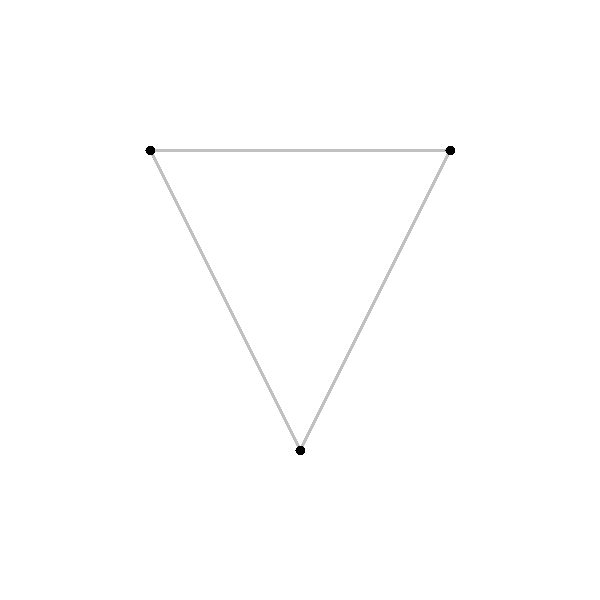
\includegraphics[width=\textwidth]{images/ExampleNetwork.png}
         \caption{Corresponding simulation image}
         \label{fig:example_network_vis}
    \end{subfigure}
    \caption{A triangular road network encoded as a file and visualised}
    \label{fig:example_network}
\end{figure}

\subsection{Agent Specification}
The program has two agent archetypes: the \textit{Car} and the \textit{Overseer}. Cars are the primary agent in the system and the subjects of the evacuation, they are modelled as point objects, but they have virtual dimensions according to a parameter. Overseer agents are those agents which do not necessarily have a contextual counterpart in the simulation, as their roles are to implement real-time features in the simulation. It is an Overseer which will implement evacuation strategies and control the scenario of the simulation. Unless stated otherwise, usages of the word \textit{agent} will refer to cars.

When a car is initialised, it is randomly distributed to a source node. On initialisation, cars calculate their shortest path to a goal node using the A* search algorithm \cite{Hart1968APaths}. In the age of smartphones and satnav this assumption is appropriate. Traffic behaviour is governed by the N-S algorithm, but the specific parameters that adjust driving behaviour are configurable. The list of car driving parameters is:

\begin{itemize}
    \item Speed Limit
    \item Acceleration
    \item Vehicle buffer - The space kept between cars (their effective lengths)
    \item Perception Radius - The distance at which a car can perceive its surroundings
\end{itemize}

Evacuation strategies - namely throttling and agent-greed - are to be implemented according to their definitions in Chapter \ref{ch:background}, and be toggle-able within the system. Each strategy's parameters are also highly configurable.

\subsection{Simulation Configuration}
A full list of configurable parameters, and their definitions, is given in Appendix \ref{appendix:parameters}. With such numerous variables, the project demands an easy method for researchers to set up a new scenario, test it, and set up an experiment that evaluates the effect of one or more independent variables on clearance time. As with the network topology, it is impractical to set up every new scenario within the system code itself, therefore it is fitting to use an external configuration file. Hence, a simulation requires two files to run, a configuration file and a network file. As all parameters are arbitrary and configurable, the simulation is agnostic towards which units are used for each variable as long as all variable units are consistent with each other. For example, if the researcher wants to configure velocity in miles per hour, distances must be given in miles to avoid unit errors - this is intuitive for any system that does not explicitly design for conflicting units. Unless specified, all default parameters are to be interpreted as SI units where applicable.

\section{Experiment Specification}

As stated in Chapter \ref{ch:background}, the metric to consider for every simulation run is \textit{clearance time} - the total time elapsed between the first evacuee leaving their source to the last evacuee reaching their destination.

Research in this area is naturally sequential. Hypotheses are built on the findings of previous experiments, which motivate the formulation of the next scenario to put to simulation. See the experiments section for a detailed analysis of the sequential experimentation process.

Initially, experiments on the effectiveness of throttling by Madireddy et al. (2011) will be replicated, and if necessary, the effect of throttling will be evaluated across different networks and under different simulation configurations.

Regarding agent greed, Zhang et al. (2009) do not explore whether the \textit{greedy threshold} of an agent, the congestion level a road must reach for an agent to choose to divert its route, shares any clear relationship with clearance time. This relationship is evaluated in Chapter \ref{ch:experimentation}.

\chapter{Design}
\label{ch:design}
\section{Mason}

At the inception of the project, an initial focus was put towards experimentation. As the project continued this focus became balanced more evenly between empirical investigation and the engineering of the system itself, however at the outset it was evident that one of the multi-agent frameworks covered in Chapter \ref{ch:background} would be a solid foundation upon which to build the simulation.

MASON (Multi-Agent Simulation of Neighbourhoods, or Networks) is a versatile Java library for providing the key architecture in agent-based applications. MASON provides a range of environment representations, or \textit{fields} in MASON nomenclature, and a GUI system that intuitively visualises system components that interact in and with the MASON fields.

This project did not tie itself heavily to MASON's broad range of features. MASON only provided a very lightweight framework to act as a foundation for the simulation construction: MASON fundamentally revolves around a \texttt{Scheduler}, object. The Scheduler is a decorated priority queue. For an agent to act in the system it must inherit the \code{Steppable} interface, which guarantees the agent has a \code{step()} method. Agents are queued into the Scheduler for each time step, and the Scheduler executes the agent's step method when it reaches the top of the queue. In compliment with this simple functionality, the Scheduler will step higher priority agents first and will step agents of equal priority in a uniformly random order.

In addition to the Scheduler, MASON's other contribution to the project was providing a GUI, and MASON's GUI-compliant graph data structure functionality. MASON Networks are a simple collection of arbitrary user-defined objects to use as nodes, and a map between nodes and their associated Edge objects. While MASON expects users to provide a class to act as a node, it provides its own Edge class. Edge objects store a `from node', `to node' and an arbitrary user-defined child object, which is expected to store semantic data about what the Edge represents. MASON Networks hence act as wrappers for user-defined node and edge objects - to that end, \code{Junction} objects were defined as the Network's node objects, and \code{Road} objects were constructed to provide a semantic representation of roads in the simulation. The driving reason for using a MASON network rather than constructing a graph directly from the \code{Junction} and \code{Road} objects is the ease of the MASON network integration with MASON's own GUI and visualisation tools.


\section{System Overview}

At the highest level, the project is composed of a simulation package, and classes which leverage it. Figure \ref{fig:system_overview} gives a simple class-relationship diagram of the system which articulates this high-level split as well as portraying a lower level system composition; the simulation package consists of a set of agents, a collection of environment classes, a pair of classes for implementing the A* algorithm, and most importantly, the \code{CoreSimulation} class.

\begin{figure}
    \centering
    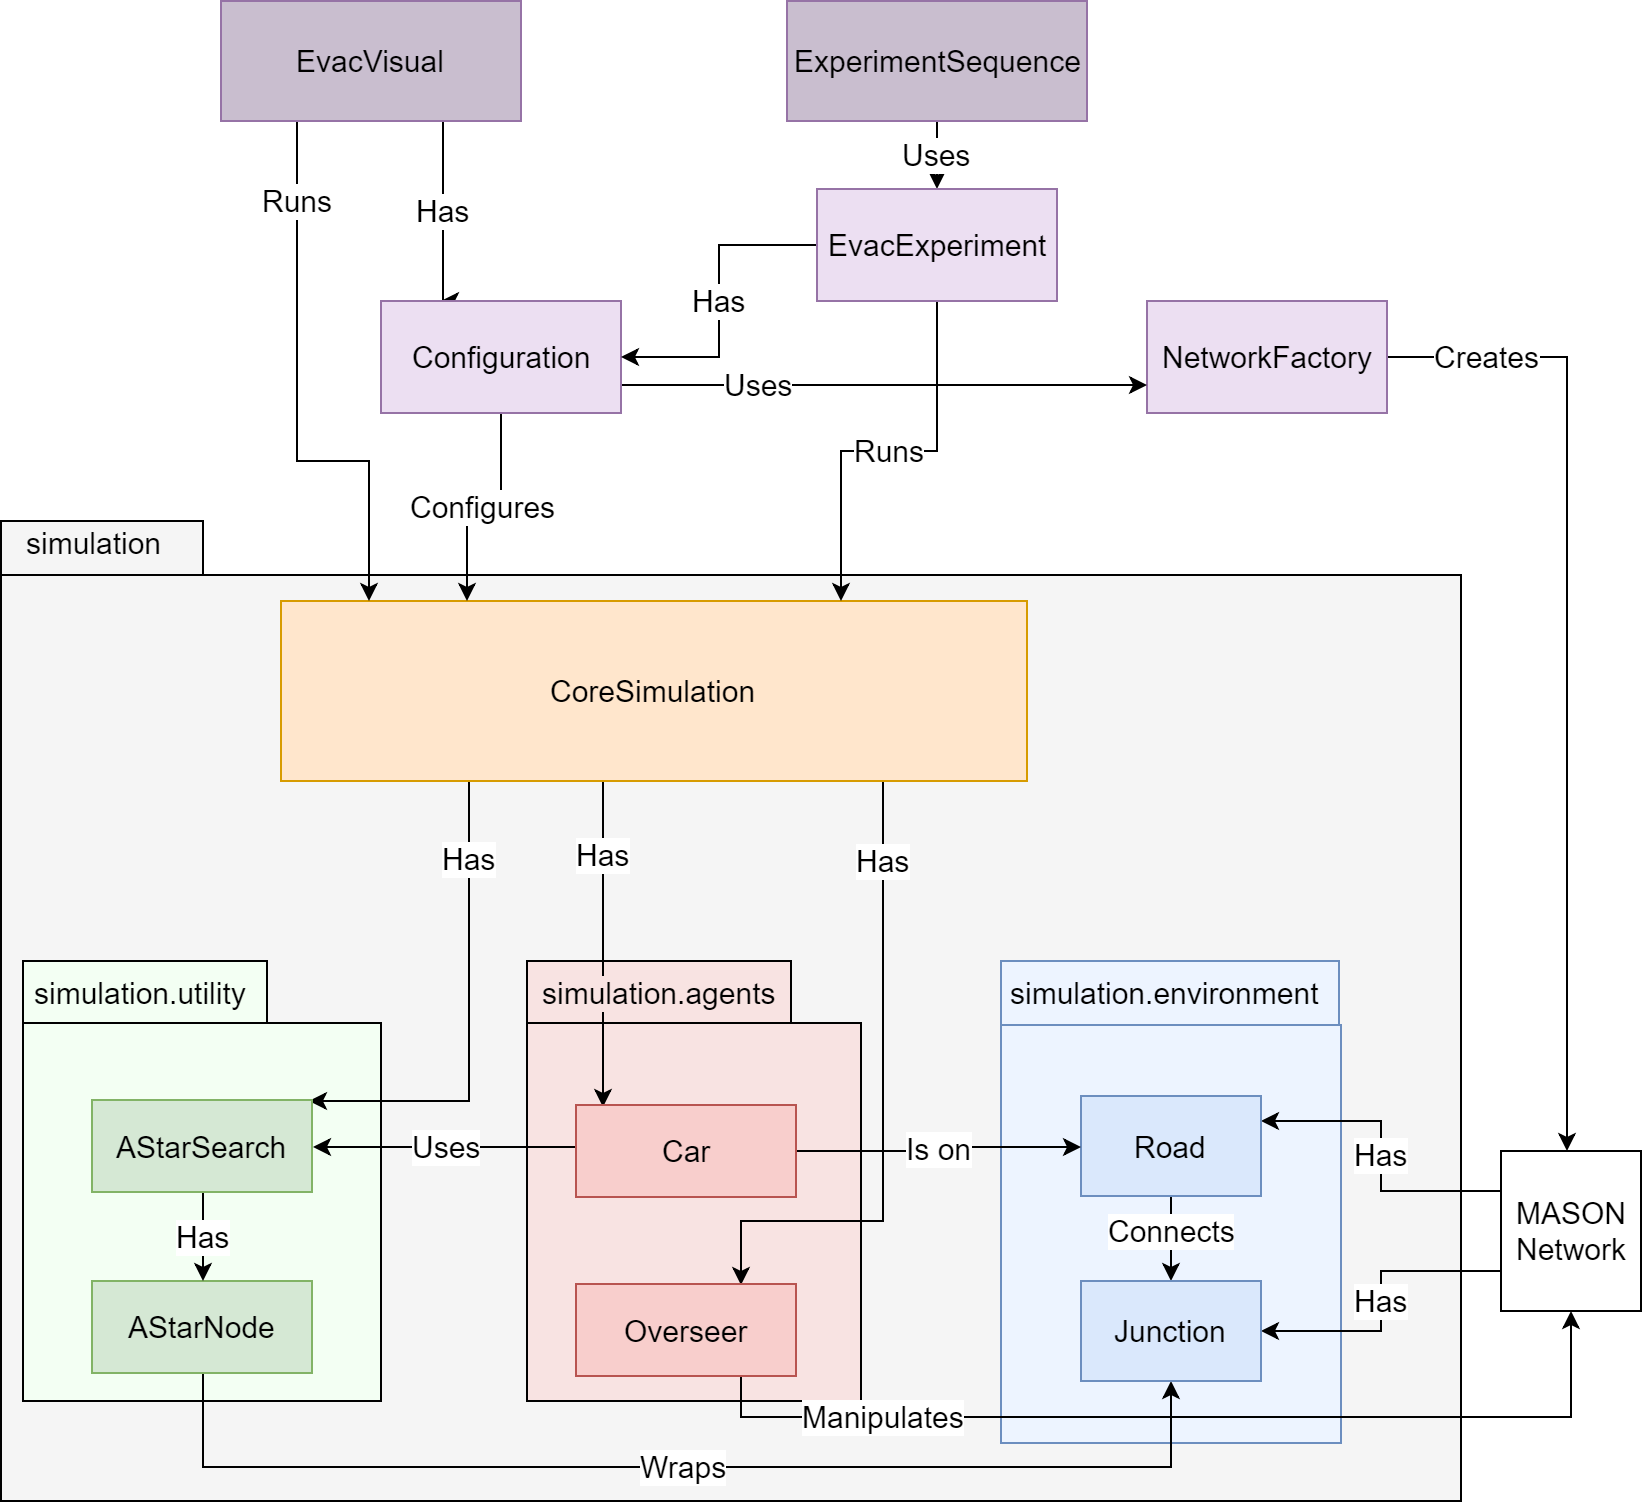
\includegraphics[width=0.95\linewidth]{images/system_overview.png}
    \caption{Project component relationship diagram}
    \label{fig:system_overview}
\end{figure}

TABLE OF CLASSES

\chapter{Implementation}
\label{ch:implementation}
Cars are modelled as individual agents, the \code{Car} class inherits MASON's \code{Steppable} interface which allows Cars to be treated as agents by the simulation's Scheduler and have their \code{step()} method called at every timestep in the simulation. Here we will discuss the \code{step()} method, what it does, and why. First though, we must understand how an agent percieves the world around it.

Modern processors no longer necessitate using CA environments in ABM, allowing continuous systems to simulate emergent behaviour with a greater spatial fidelity. Agents in this model exist in such a continuous 2D space, but this presents challenges. Most trivially, the N-S algorithm must be adapted to work for continuous environments, however this is easily overcome as the design of N-S does not strictly require a discrete coordinate space to function. Adapting the N-S algorithm merely requires an adjustment to cases where the agent must slow down due to another car in front of it. Where discrete N-S slows an agent down so that it comes to occupy the cell immediately behind the cell of the car in front of it, continuous N-S slows the same agent down so that its position is some arbitrary stopping distance behind the car in front of it.

A more difficult problem brought about by the environment is implementing agents that follow the roads, and designing how an agent will process nearby cars into its own perception of the road ahead. The solution to this problem is found by giving agents access to the real, 2D, global space as well as a second \textit{network space} within which they can process their surroundings.

\subsection{Network Space}

Network space is a \textit{one-dimensional} coordinate system defined by an agent's current position along the length of a 1D vector of a road segment, we shall call this current length along a road the \textit{index}. Network space is best understood using an example, with Figure \ref{fig:network_space} for reference:

\vspace{1cm}
\begin{figure}[ht]
    \centering
    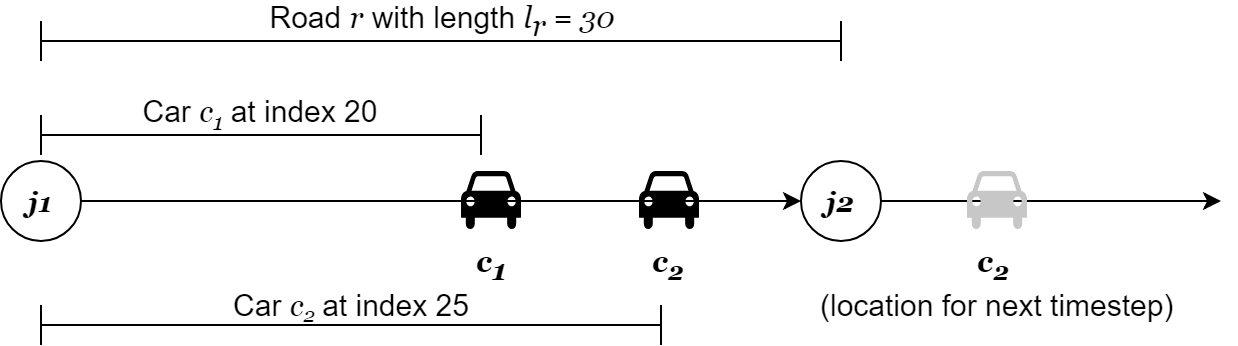
\includegraphics[width=0.8\textwidth]{images/network_space.png}
    \caption{Network Space road traversal}
    \label{fig:network_space}
\end{figure}
\vspace{1cm}
Let $r$ be a road of length $l_r$ = 30 units, directed from a junction $j_1$ towards a junction $j_2$. Suppose a car $c_1$ is positioned 20 units along the road, then the \textit{index} of $c_1$ on $r$ is equal to 20. Suppose the next car ahead of $c_1$, being $c_2$, is 5 units in front, the index of $c_2$ on $r$ is equal to 25. By definition, if the index of a car on road $r$ reaches $l_r$ then that car must have traversed the length of the road and reached the road's destination node, $j_2$.

Here we have been able to reduce a car's two dimensional road behaviour to one dimension. In compliment with the network space, cars still exist in and move through the global 2D space - this facilitates agents that are able to perceive and react not only to the roads but also any other feature in their vicinity. None of the experiments in the scope of this project take advantage of this capability, but potential applications of the feature include allowing cars to interact with pedestrians in the 2D space, and programming cars to react to seeing fire or some other hazard anywhere in the environment. 

As cars move through network space, a transformation is needed to calculate their location in global space. For a car, $c$ at a network space index $i$ on a road $r$ of length $l_r$ from junction $v$ to junction $w$, the global space position of $c$, $p_c$, is given by:

\begin{equation}
    p_c \;=\; v + i\cdot\hat{vw} \;=\; v + i(\frac{\vec{vw}}{l_r})
    \label{eq:vector_global}
\end{equation}

The $x$ and $y$ coordinates of $c$ are found by separating equation \ref{eq:vector_global} into its $x$ and $y$ components:

\begin{equation}
    x_c \;=\; v_x + i(\frac{x_w - x_v}{l_r})
    \label{eq:vector_global}
\end{equation}

\begin{equation}
    y_c \;=\; v_y + i(\frac{y_w - y_v}{l_r})
    \label{eq:vector_global}
\end{equation}

\subsection{Traversing Network Space}
Returning to our earlier example of network space: if $c_2$, which is at index 25, has a velocity greater than 5 in the current timestep then its new index must exceed the length of road $r$, therefore it must travel through the junction $j_2$ and travel onto the next road segment with some residual movement as seen in Figure \ref{fig:network_space}. This next road segment is determined by the evacuation route which $c_2$ had previously calculated to reach its evacuation destination. Hence the general idea of an agent's \code{step()} algorithm falls into place:

\vspace{0.5cm}
\begin{algorithm}[H]
    \SetKwData{Overbreaking}{overbreakingFactor}
    \SetKwFunction{NextCar}{DistanceToNextCar}
    \SetKwFunction{NextEdge}{MoveToNextEdge}
    \SetKwFunction{Location}{CalculateLocation}
    \SetKwFunction{Max}{Max}
    // Adapted N-S Algo:
    
    \uIf{$velocity < speed\_limit$}{
        $velocity \leftarrow velocity + acceleration$\;
    }
    
    \uIf{$\NextCar{car} < velocity$}{
        $velocity \leftarrow \NextCar{car} - bufferBetweenVehicles$\;
    }
    
    \uIf{with probability p}{
        $velocity \leftarrow velocity - overbreakingFactor$\;
    }
    $velocity \leftarrow \Max{0,velocity}$\;
    
    // N-S algo ends
    \BlankLine
    $index \leftarrow index + velocity$\;
    \uIf{$index > roadLength$}{
        $residualMovement \leftarrow index-roadLength$\;
        \NextEdge{residualMovement}\;
    }
    
    \Location{}\;
    
    \caption{A naïve car step method}
    \label{alg:naive_step}
\end{algorithm}
\vspace{0.5cm}


In Algorithm \ref{alg:naive_step}, the \code{MoveToNextEdge()} psuedocode method would perform the necessary steps to load an agent onto a new road segment and it would check if the residual movement is great enough that the agent would traverse the entirety of the new road in a single step. In such a case, \code{MoveToNextEdge()} will be called again with whatever remainder of the step movement is to carry forward to the \textit{next} road segment. This will occur of road segments are exceptionally small and an agent can traverse multiple edges in one time step. As agents are called in random sequence, if an unexpected car joins the agent's route at an upcoming junction, it will be perceived by the agent during their step method. 

It is imperative that \code{DistanceToNextCar()} finds the distance to the next car on the route, regardless of how many roads away such a car is. A first implementation of the agent's naïve step only searched for a next car on the current road segment, however this broke down if no neighbour was found but a neighbour existed at a very low index on the \textit{next} road; the agent would move to the next road and either completely skip over the car which was supposed to be in front of it, or if it tried to leave a buffer between it and the newly found neighbour, it would have to reverse the process of moving edge and replace itself on the old edge. To avoid excessive loading and unloading of agents onto roads, the agent looks ahead in its route for the next neighbour. In practicality, the source code is far more complex than Algorithm \ref{alg:naive_step} and the proper Java method \code{Car.calculateDistanceToNeighbour()} which realises the functionality of this psuedocode method and uses a perception distance outside of which an agent cannot see, hence the search for a next neighbour is bounded.


\subsection{Adding Complexity}

The Naïve Step algorithm works for all simple driving models, however the algorithm fails when complexity is introduced to the car-agent's decision making process, such as when agent greed and road throttling are introduced.

Maths for interpolation n tings
    
Initial loading onto network error

\chapter{Experimentation}
\label{ch:experimentation}
\section{N-S driving evaluation}

we gucci

\section{throttling}

My madireddy results are more intuitive than Madireddy's
UT=LT makes for optimal flow as the road operates on a 1-in-1-out basis

\section{Greed}

\subsection{Proportion of pop}

Redo. Had no trend but I did the experiment at greedy threshold = 0
Try redo at greedy threshold = 0.2 or whatever is optimal for that particular population size 

\subsection{greedy threshold}
A zero greedy threshold, while incredibly unrealistic, will cause agents to divert from their planned route and seek out a new route at every junction, regardless of congestion level. Contrastingly, a greedy threshold of $1$ will only direct an agent to seek a new route if their current route is maximally congested. It is hypothesised that there is a greedy threshold which will minimise the clearance time of a road network.

optimal greedy threshold seems to depend on population size

Need to take base (no greedy decisions) measurement for all populations as well!


\chapter{Discussion}
\label{ch:discussion}
Discussion. Here you will summarise your achievements and also the deficiencies of your project. You can also say what you would or could have done, if you had had more time or if things had worked out differently. It is important to be completely honest about the deficiencies and inadequacies of your work, such as they are. Part of your aim is to demonstrate your ability to recognise problems that remain.

\chapter{Conclusion}
\label{ch:conclusion}
\input{chapters/conclusion.tex}

\printbibliography

\appendix
\chapter{Structure of Project Directory}
\label{appendix:directory}
\input{appendicies/directory.tex}

\chapter{List of Configurable Parameters}
\label{appendix:parameters}
\input{appendicies/parameters.tex}

\chapter{Complete System Class Diagram}
\label{appendix:class_diagram}
\input{appendicies/class_diagram.tex}

\end{document}